\PassOptionsToPackage{fontset=none}{ctex}
\documentclass[withoutpreface,bwprint]{cumcmthesis}
\usepackage{cumcm2026}
\usepackage{amsmath,amssymb,mathtools,booktabs,tabularx,longtable,multirow}
\usepackage{graphicx,float,caption,subcaption,enumitem,siunitx,hyperref,fvextra,needspace}
\setCJKmainfont[BoldFont=SimHei,ItalicFont=KaiTi]{SimSun}
\setCJKsansfont[BoldFont=SimHei]{SimHei}
\setCJKmonofont{SimSun}
\setCJKfamilyfont{zhsong}[BoldFont=SimHei]{SimSun}
\setCJKfamilyfont{zhhei}[BoldFont=SimHei]{SimHei}
\providecommand{\heiti}{\CJKfamily{zhhei}}
\providecommand{\songti}{\CJKfamily{zhsong}}
\renewcommand{\thesection}{\arabic{section}}
\renewcommand{\thesubsection}{\thesection.\arabic{subsection}}
\renewcommand{\thesubsubsection}{\thesubsection.\arabic{subsubsection}}
\clearcaptionsetup{sub}
\titleformat{\section}{\centering\heiti\zihao{4}}{\thesection}{0.8em}{}
\titleformat{\subsection}{\heiti\zihao{-4}}{\thesubsection}{0.8em}{}
\titleformat{\subsubsection}{\heiti\zihao{-4}}{\thesubsubsection}{0.8em}{}
\hypersetup{hidelinks}
\setlength{\emergencystretch}{2em}
\raggedbottom
\title{考虑药材内部实际温度场的热湿传递与收缩移动边界模型}
\tihao{A}\baominghao{}\schoolname{}\membera{}\memberb{}\memberc{}\supervisor{}
\yearinput{2026}\monthinput{9}\dayinput{13}
\newcommand{\kgkg}{\ensuremath{\mathrm{kg/kg}}}
\newcommand{\Rtime}{R(t)}
\newcommand{\Cmax}{C_{\max}}

\begin{document}
\maketitle

\begin{abstract}
针对圆柱形药材烘干中“表面先变、内部滞后、长期收缩”的特征，本文在保留题设物性关系的基础上，重新构建一条独立的计算路线：问题二至四不再把药材内部温度直接设为烘房温度，而是同步求解显热传导方程，并将预测温度场反馈给含水率扩散系数。问题一沿用二维轴对称热湿模型作为短时基线，问题四进一步在半径观测驱动的收缩移动域中推进。

数值上采用轴对称有限体积法、后向欧拉时间推进和 Picard 非线性迭代；外边界使用传热、传质串联阻力，Q4 使用保形插值的半径函数和干固体质量守恒。新版计算的主结果为：Q2 在 3 h 时中心和表面温度分别为 49.8504\(^{\circ}\mathrm C\) 与 49.9670\(^{\circ}\mathrm C\)，全域最大含水率为 1.76623\,\kgkg；Q3 首次低于安全阈值的插值时刻为 207158.1 s，按 60 s 口径报告 207180 s（57.55 h）；Q4 相应为 184080 s（51.13 h）。Q2 的径向剖面显示，温度梯度消失前表面失水明显快于中心，说明内部温度场不能仅作为装饰性变量。

现有附件足以计算“不含潜热的显热温度场—水分扩散”模型，但不足以唯一确定含汽化潜热的模型：尚缺潜热或相变焓、蒸发动力学/平衡关系以及气相传输参数。因而本文把内部温度称为模型预测量，明确给出适用边界，不将其表述为实验真实温度。
\keywords{药材烘干\quad 内部温度场\quad 轴对称有限体积\quad 状态相关扩散\quad 收缩移动边界}
\end{abstract}

\section{问题重述与新版目标}
药材可近似为长圆柱体。附件 1 给出烘房温度与表面水分边界，附件 2 给出长期半径观测。题目要求求出短时温度/含水率分布、状态相关物性下的含水率变化、固定域达标时间以及考虑收缩后的达标时间。原论文在问题二至四中采用了 $T=T_\infty(t)$ 的内部温度简化。根据复核意见，本版的改动目标是：保留原论文及原程序不动，另建独立目录，用同一组外部数据求解内部显热温度，并把它作为问题二至四的主模型。

本文只把“可由已有数据闭合”的显热温度场纳入重新计算，不擅自补写潜热参数。这样既能回答内部实际温度对干燥轨迹的影响，也能清楚说明仍然存在的数据缺口。

\section{数据、假设与可计算性审计}
\subsection{数据与边界}
初始温度为 $T_0=301.15\,\mathrm K$，初始干基含水率为 $C_0=2.55\,\kgkg$，圆柱长度 $L=0.25\,\mathrm m$，初始半径 $R_0=0.02\,\mathrm m$。传热系数取 $h=25\,\mathrm{W/(m^2\,K)}$，传质系数取 $h_m=8\times10^{-7}\,\mathrm{m/s}$。附件 1 在 $0$--$4$ h 内的环境序列采用分段线性插值；4 h 后采用末一小时平均值恒定延拓。Q4 半径序列采用 PCHIP，超出观测末点后保持末值。

\begin{table}[H]\centering
\caption{本版温度场模型的数据闭合审计}\label{tab:data-audit}
\begin{tabularx}{0.96\linewidth}{p{0.24\linewidth}X p{0.18\linewidth}}
\toprule
模块&已有数据&状态\\\midrule
显热传导&$T_0,T_\infty(t),\rho(C),c_p(C),k(C),h,L,R(t)$&可计算\\
水分扩散&$C_0,C_\infty(t),D(C,T),h_m$&可计算\\
含潜热模型&$L_v(C,T)$、相变速率或气液平衡关系&缺失\\
气相输运&内部蒸汽分压、孔隙率、渗透率等&缺失\\
实验验证&内部多位置温度/含水率时序&缺失；限制真实性判断\\
\bottomrule
\end{tabularx}\end{table}
表\ref{tab:data-audit} 的审计结果决定了本文只计算无潜热显热温度场；收缩建模所需的质量守恒处理与相关研究中的思路一致\cite{p04}。

\subsection{模型假设}
药材连续、均质、轴对称，初值均匀；轴线和中截面为对称边界，侧面和端面满足 Robin 交换。所有本版结果仍不含汽化潜热、吸附热和反应热；因此“实际温度”指由显热方程预测的内部温度，而非实测温度。Q4 采用径向仿射收缩、轴向长度不变、干固体质量守恒。4 h 后的环境延拓是计算假设，不是未来实测数据。

\section{热湿耦合模型}
\subsection{固定域轴对称方程}
在半域 $\Omega=\{(r,z):0\le r\le R(t),0\le z\le L/2\}$ 上，含水率满足
\begin{equation}
\frac{\partial C}{\partial t}=\frac1r\frac{\partial}{\partial r}\left(rD(C,T)\frac{\partial C}{\partial r}\right)+\frac{\partial}{\partial z}\left(D(C,T)\frac{\partial C}{\partial z}\right).
\label{eq:mass}
\end{equation}
温度由显热方程给出
\begin{equation}
\rho(C)c_p(C)\frac{\partial T}{\partial t}=\frac1r\frac{\partial}{\partial r}\left(rk(C)\frac{\partial T}{\partial r}\right)+\frac{\partial}{\partial z}\left(k(C)\frac{\partial T}{\partial z}\right).
\label{eq:heat}
\end{equation}
外边界为
\begin{equation}
-D\nabla C\cdot\boldsymbol n=h_m(C_s-C_\infty),\qquad -k\nabla T\cdot\boldsymbol n=h(T_s-T_\infty),
\label{eq:robin}
\end{equation}
轴线和中截面取零法向通量。与旧路线的差异集中在式 \eqref{eq:heat}：本版把 $T(r,z,t)$ 作为状态量求解，再在每个非线性迭代中更新 $D(C,T)$；旧路线的 $T=T_\infty(t)$ 仅作为控制组保留。

Q2、Q3 的物性为
\begin{equation}
\rho=650+128C,\quad c_p=1450+\frac{2736C}{C+1},\quad k=0.21+\frac{0.38C}{C+1},
\end{equation}
\begin{equation}
D=2.4\times10^{-3}\exp(-0.45/C)\exp(-3850/T),
\label{eq:q23}
\end{equation}
Q4 使用题设给定的另一组关系
\begin{equation}
\rho=760+90C,\quad c_p=1850+\frac{2150C}{C+1},\quad k=0.12+\frac{0.20C}{C+1},
\end{equation}
\begin{equation}
D=4.2\times10^{-4}\exp(-0.30/C)\exp(-3850/T).
\label{eq:q4}
\end{equation}
温度在指数项中始终使用 K。

\subsection{守恒离散与事件判据}
对环柱控制体积分，体积为
\begin{equation}
V_{ij}=\pi(r_{i+1/2}^2-r_{i-1/2}^2)(z_{j+1/2}-z_{j-1/2}).
\end{equation}
内部界面采用扩散系数调和平均，边界把半单元扩散阻力与对流阻力串联。后向欧拉格式的含水率更新写为
\begin{equation}
\frac{V_P}{\Delta t}(C_P^{n+1}-C_P^n)=\sum_NG_{PN}(C_N^{n+1}-C_P^{n+1})+\sum_bG_b(C_\infty^{n+1}-C_P^{n+1}).
\label{eq:fv}
\end{equation}
温度方程采用同一通量组装，仅将库存项换为 $\rho c_pV$、扩散系数换为 $k$。每步交替进行 Picard 迭代，线性相对残差控制在 $5\times10^{-11}$ 以内。Q4 在当前半径下更新控制体几何和干固体密度；其全域达标条件为
\begin{equation}
\max_{\Omega(t)}C<0.15-10^{-6}.
\label{eq:event}
\end{equation}
以首次越过阈值的相邻时间步做线性插值，再向上取整到 60 s。

图\ref{fig:schematic} 将新版主路线中的半域、对称边界、移动侧面和热湿边界通量统一画出，便于区分内部状态量与外部边界量。
\begin{figure}[H]\centering
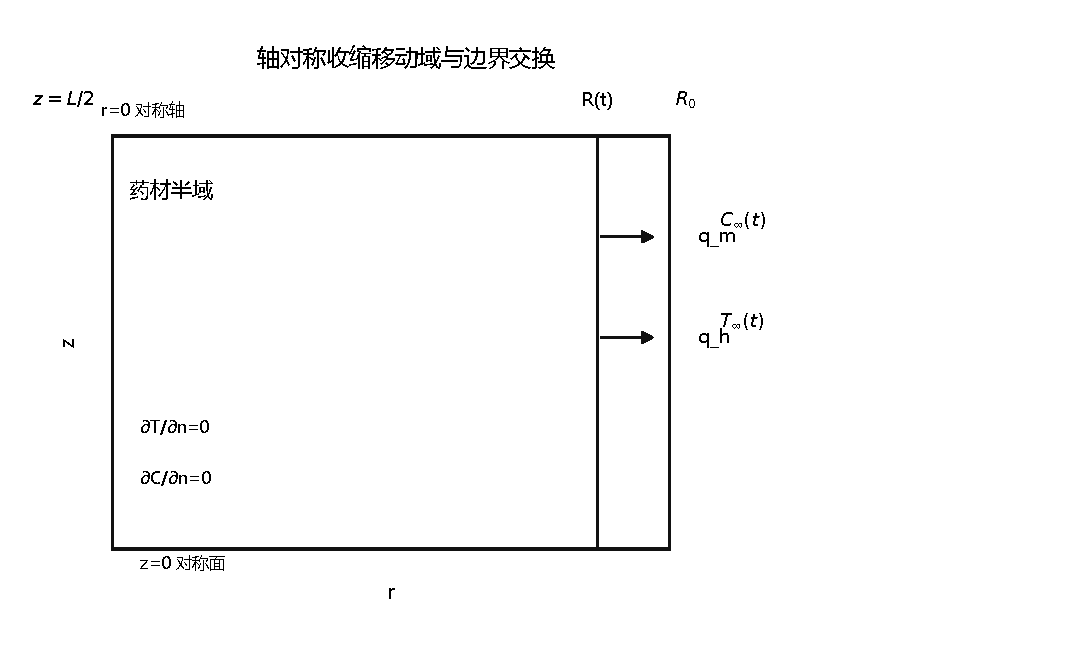
\includegraphics[width=0.92\linewidth]{figures/FIG-TEMP-FIELD-MODEL-SCHEMATIC}
\caption{新版内部温度场与含水率场的轴对称收缩移动域示意图}\label{fig:schematic}
\end{figure}

\section{问题一：短时二维基线}
问题一采用题设常量热物性和给定的 $D(C)$，分别计算一维径向和二维轴对称场。1800 s 时二维模型中截面轴心温度为 33.5763\(^{\circ}\mathrm C\)，表面为 36.7859\(^{\circ}\mathrm C\)，平均含水率为 2.2750\,\kgkg；一维模型平均含水率为 2.2936\,\kgkg。端面提供额外传质通道，使二维平均值降低。图\ref{fig:q1-field} 为中截面场量，图\ref{fig:q1-end} 为端面效应对照。
\begin{figure}[H]\centering
\includegraphics[width=0.92\linewidth]{figures/FIG-Q1-C-FIELD.pdf}\caption{问题一中截面含水率场}\label{fig:q1-field}\end{figure}
\begin{figure}[H]\centering
\includegraphics[width=0.92\linewidth]{figures/FIG-Q1-END-EFFECT.png}\caption{问题一端面效应对照}\label{fig:q1-end}\end{figure}

\section{问题二：内部温度场下的 3 h 过程}
\subsection{温度场结果}
采用 $140\times36$ 个控制体、$\Delta t=5$ s，从均匀初值重新积分至 3 h。图\ref{fig:q2-temp} 给出了中截面轴心与表面温度。表面先升温，中心存在明显热滞后；3 h 时差值约 0.1166\(^{\circ}\mathrm C\)，温度差虽已变小，但早期差异会通过式 \eqref{eq:q23} 影响扩散系数。
\begin{figure}[H]\centering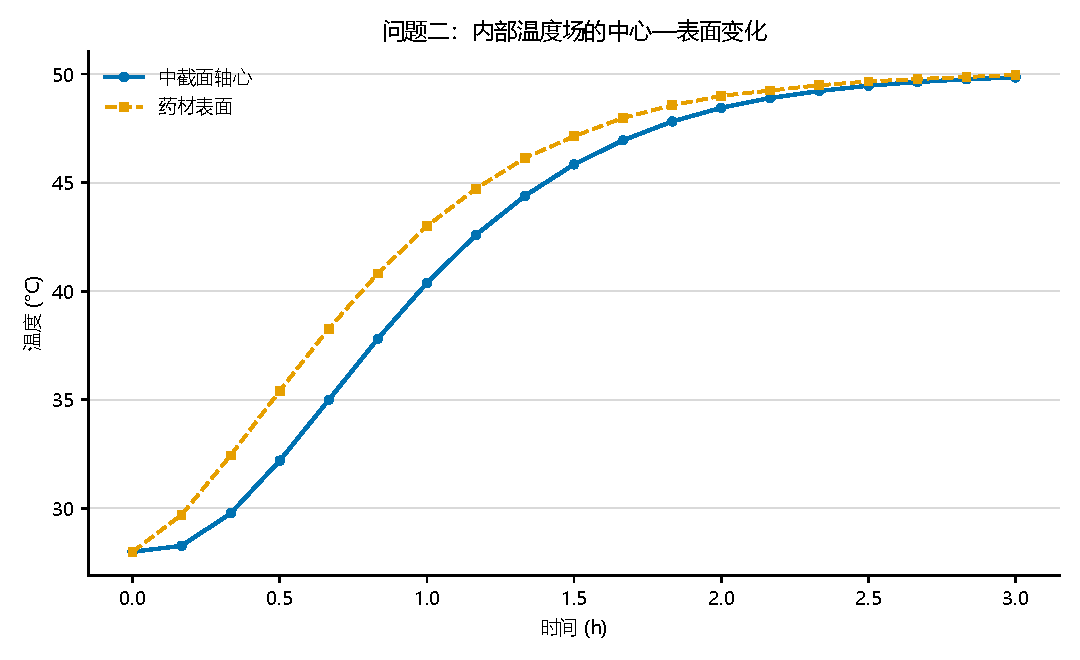
\includegraphics[width=0.92\linewidth]{figures/FIG-TEMP-FIELD-Q2-TEMP}\caption{问题二内部温度场的中心—表面轨迹}\label{fig:q2-temp}\end{figure}

\begin{table}[H]\centering\caption{问题二内部温度场的代表性输出}\label{tab:q2-result}
\begin{tabular}{c c c c c}\toprule
时间/h&中心温度/\(^{\circ}\mathrm C\)&表面温度/\(^{\circ}\mathrm C\)&全域最大 $C$&体积平均 $C$\\\midrule
0.5&32.1968&35.4177&2.5499&2.2632\\
1.0&40.3819&43.0000&2.5254&2.0322\\
1.5&45.8442&47.1379&2.3857&1.8264\\
2.0&48.4491&49.0025&2.1707&1.6413\\
2.5&49.4670&49.6624&1.9566&1.4755\\
3.0&49.8504&49.9670&1.7662&1.3277\\
\bottomrule\end{tabular}\end{table}
表\ref{tab:q2-result} 中的中心—表面温差直接来自热方程的解，而不是将环境温度复制到全部单元；这也是传热与传质耦合研究中需要分别检查内部场和边界交换的原因\cite{p06,p11}。

\subsection{含水率剖面与路线对照}
图\ref{fig:q2-profiles} 在六个时刻给出中截面径向剖面。早期表层梯度最大，随后梯度向中心推进；因此只报告表面含水率会高估全域干燥程度。图\ref{fig:q2-compare} 将旧的“烘房温度”控制组与新版内部温度场路线并列。三条曲线的网格和时间步不完全相同，图中只作机制对照，不作精度排序。
\begin{figure}[H]\centering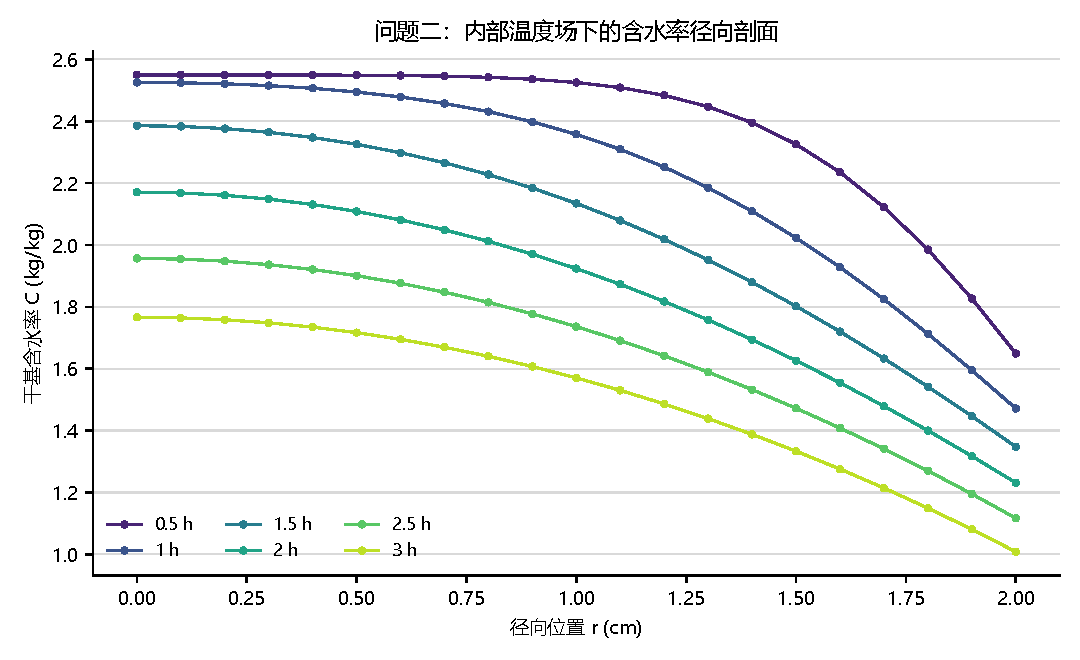
\includegraphics[width=0.92\linewidth]{figures/FIG-TEMP-FIELD-Q2-PROFILES}\caption{问题二内部温度场下的含水率径向剖面}\label{fig:q2-profiles}\end{figure}
\begin{figure}[H]\centering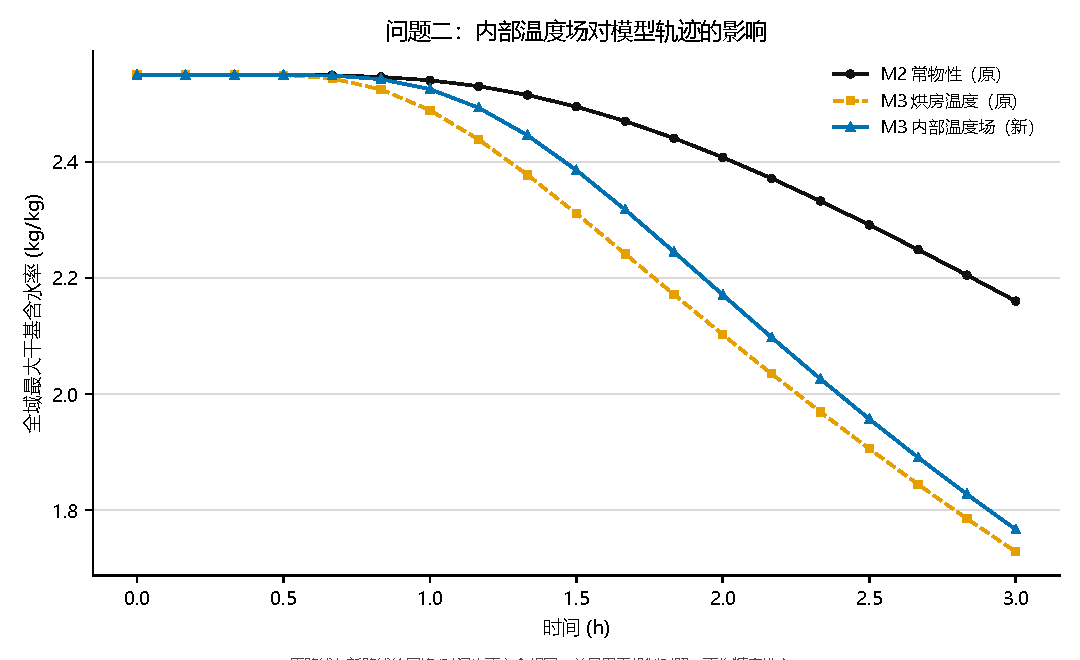
\includegraphics[width=0.92\linewidth]{figures/FIG-TEMP-FIELD-Q2-COMPARE}\caption{内部温度场路线与旧控制路线的轨迹对照}\label{fig:q2-compare}\end{figure}

\section{问题三：固定域全域达标时间}
问题三从 $t=0$ 重新积分。采用 $140\times36$ 网格和 $\Delta t=60$ s，4 h 后按末段平均环境延拓。首次越过式 \eqref{eq:event} 的插值时刻为 207158.1 s，按 60 s 口径报告为 207180 s，即 57.55 h。末步的中心和表面温度均为 49.9989\(^{\circ}\mathrm C\)，说明到长期达标时热滞后已基本消失，但它仍改变了早期扩散历史。图\ref{fig:q3} 给出轨迹与插值事件。
\begin{figure}[H]\centering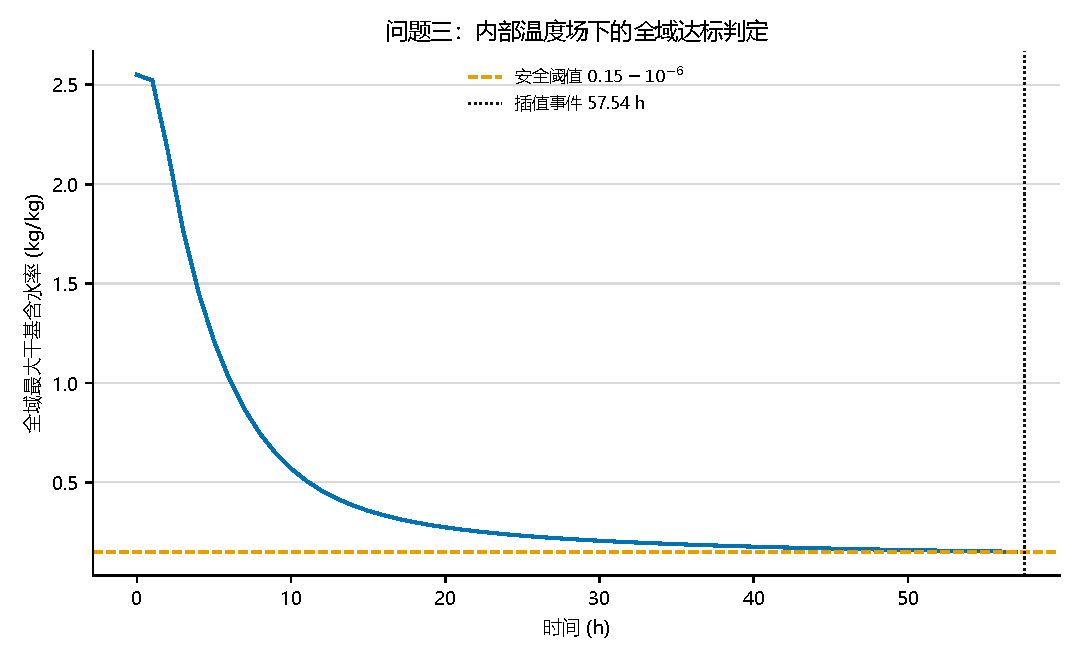
\includegraphics[width=0.92\linewidth]{figures/FIG-TEMP-FIELD-Q3-THRESHOLD}\caption{问题三内部温度场下的全域达标判定}\label{fig:q3}\end{figure}

\section{问题四：收缩移动域下的达标时间}
Q4 使用附件半径序列构造 $R(t)$，在每个时间步更新移动控制体、干固体密度和 Q4 物性。图\ref{fig:q4-radius} 显示半径从 2.00 cm 向 1.20 cm 收缩；这既缩短扩散距离，也改变边界面积和库存权重，不能只用距离平方比例修正。
\begin{figure}[H]\centering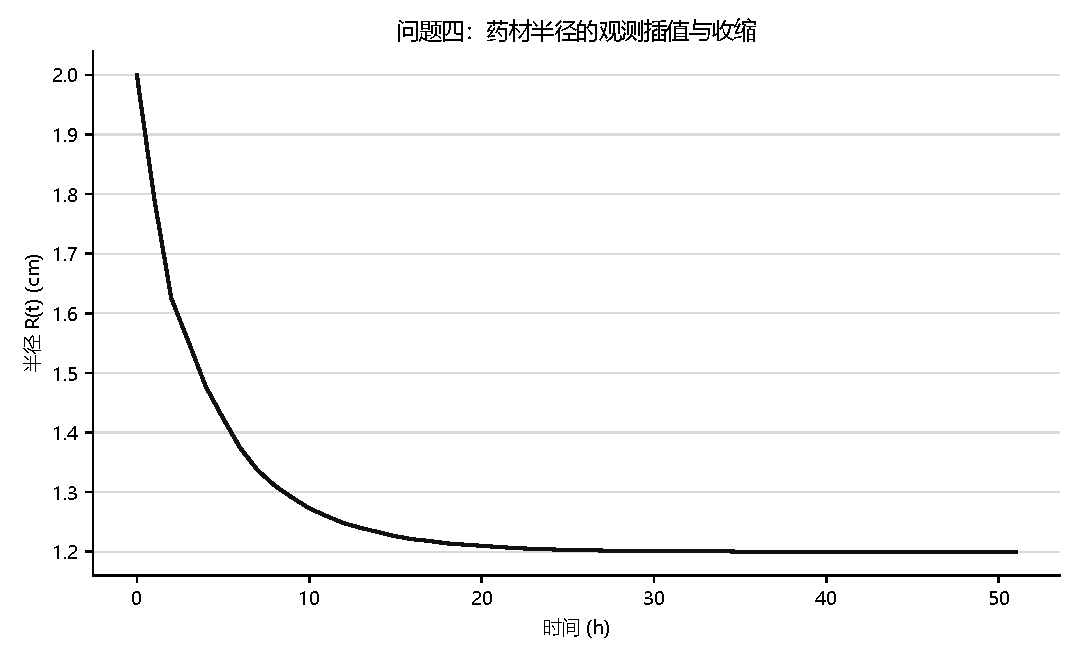
\includegraphics[width=0.92\linewidth]{figures/FIG-TEMP-FIELD-Q4-RADIUS}\caption{问题四半径观测插值与收缩轨迹}\label{fig:q4-radius}\end{figure}
首次越过阈值的插值时刻为 184079.97 s，报告时刻为 184080 s，即 51.13 h。图\ref{fig:q4} 给出全域最大含水率轨迹。该值与问题三的差异同时包含 Q4 物性改变和收缩几何效应，不能解释为纯收缩贡献。
\begin{figure}[H]\centering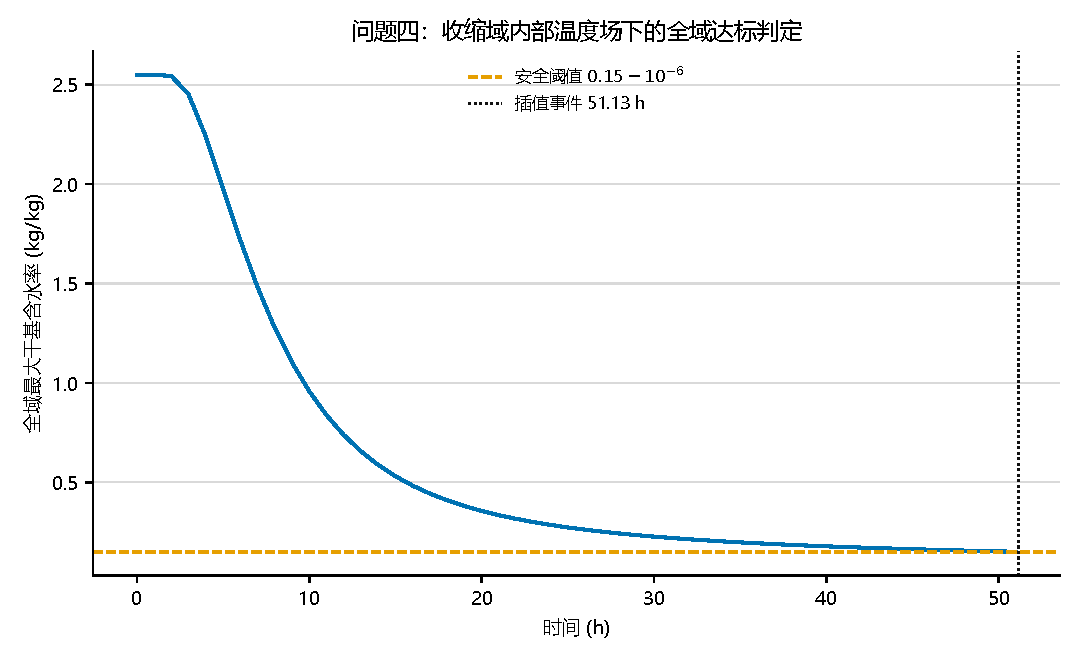
\includegraphics[width=0.92\linewidth]{figures/FIG-TEMP-FIELD-Q4-THRESHOLD}\caption{问题四收缩域内部温度场下的全域达标判定}\label{fig:q4}\end{figure}

\section{数值检验、局限与结论}
\subsection{守恒与残差}
Q2--Q4 新路线的最大线性相对残差分别为 $5.00\times10^{-11}$、$5.01\times10^{-11}$ 和 $5.01\times10^{-11}$；归一化水分平衡误差分别为 $2.02\times10^{-8}$、$1.67\times10^{-9}$ 和 $1.22\times10^{-9}$。这些数值检验说明离散方程求解充分、库存与边界通量基本闭合，但不等于实验验证，也不能消除时间步和空间网格误差。
\begin{table}[H]\centering\caption{新版计算的数值质量指标}\label{tab:checks}
\begin{tabular}{lccc}\toprule
算例&网格（径向$\times$轴向）&时间步/s&最大平衡误差\\\midrule
Q2 内部温度场&$140\times36$&5&$2.02\times10^{-8}$\\
Q3 固定域&$140\times36$&60&$1.67\times10^{-9}$\\
Q4 收缩移动域&$140\times32$&60&$1.22\times10^{-9}$\\
\bottomrule\end{tabular}\end{table}
表\ref{tab:checks} 给出可复现实验所需的网格、步长和守恒误差，结果文件中的线性残差还可由日志逐步核对。

\subsection{局限与缺失数据}
本版仍未加入潜热，因为附件没有 $L_v(C,T)$、相变速率/气液平衡关系，也没有内部蒸汽分压、孔隙率和渗透率等气相传输参数。若强行加入潜热，只能任意补参数，无法得到唯一、可审计的答案。内部多点温度和含水率观测同样缺失，因此当前温度是模型预测而不是实验事实。后续若补充这些数据，应先进行潜热参数辨识和独立批次验证，再把含潜热路线升级为主模型。

\subsection{结论}
在现有数据可闭合的范围内，本文完成了“显热内部温度场—状态相关水分扩散—收缩移动域”的新版计算。Q2 的 3 h 中心/表面温度为 49.8504/49.9670\(^{\circ}\mathrm C\)，最大含水率为 1.76623\,\kgkg；Q3、Q4 的 60 s 基准报告时间分别为 57.55 h 和 51.13 h。与旧路线相比，新版明确呈现了升温阶段的内部热滞后，并把缺失的潜热数据列为可验证的后续工作。所有结果均附带网格、时间步、边界延拓和“无潜热”限定。

\begin{thebibliography}{99}
\bibitem{p04} Mahiuddin M, Khan M I H, Kumar C, et al. Shrinkage of Food Materials During Drying: Current Status and Challenges[J]. Comprehensive Reviews in Food Science and Food Safety, 2018, 17(5): 1113--1126.
\bibitem{p06} Defraeye T, Blocken B, Carmeliet J. Analysis of convective heat and mass transfer coefficients for convective drying of a porous flat plate by conjugate modelling[J]. International Journal of Heat and Mass Transfer, 2012, 55: 112--124.
\bibitem{p11} Khan M I H, Batuwatta-Gamage C P, Karim M A, et al. Fundamental Understanding of Heat and Mass Transfer Processes for Physics-Informed Machine Learning-Based Drying Modelling[J]. Energies, 2022, 15: 9347.
\end{thebibliography}

\section*{AI工具使用声明}
本参赛队使用 AI 工具辅助代码调试、数值计算、图表制作和文字整理；模型假设、数据审计、结果复核及最终提交由参赛队负责。旧版论文和新版修订的目录、源文件及运行日志均保留在项目支撑材料中。

\clearpage
\begin{appendices}
\section{新版计算与图件文件}
新版核心程序、运行脚本、图件脚本和修订说明分别位于 \path{code-sources/}。结果 CSV 位于项目目录 \path{04-compute/revision-temp-field-20260913/results/}，包括温度轨迹、含水率轨迹、径向剖面和摘要表。修订清单 \path{revision-manifest.json} 记录源程序哈希、数据审计和缺失字段。
\section{新版核心程序（节选）}
以下为本版真正执行的显热温度场求解器及驱动程序全文。旧版完整代码附录仍保存在 \path{08-paper/范文风格重写版/}，不在此处替代新版程序。
\subsection{温度场求解器}
\VerbatimInput{code-sources/formal_compute_temp_field.py}
\subsection{批量运行脚本}
\VerbatimInput{code-sources/run_temp_field.py}
\subsection{结果固化脚本}
\VerbatimInput{code-sources/finalize_revision.py}
\subsection{新版图件脚本}
\VerbatimInput{code-sources/plot_temp_field_figures.py}
\end{appendices}
\end{document}
